\section{Gauge symmetries: a brief introduction}\label{sec:Gauge}
\textit{The formulas in this section are from book \cite{Quark_Lepton}.}
\subsection{The Lagrangian}\label{subsec:Lagrangian}

As we known, in classic physics, the motion equation of a particle can be obtained from the Lagrange's equation
\begin{equation}
\frac{d}{dt}(\frac{\partial L}{\partial \dot{q_i}}) - \frac{\partial L}{\partial q_i}=0
\label{eq:Lagrangian}
\end{equation}
where the $q_i$ are the generalized coordinates of the particle, $t$ is the time variable and $\dot{q_i}=dq_i/dt$. The $L\equiv T-V$, where $T$ is kinetic energy of the particle and $V$ is the potential energy of the particle. The Lagrange's equation \ref{eq:Lagrangian} can be extended from describing the motion of one particle to describe the motion of a field $\phi(t,\mathbf{x})$ (which has a value at every point in space that changes in time) by replace $q_i$ and $\dot{q_i}$ with $\phi$ and $\partial\phi/\partial x_\mu$ respectively, here the $x_\mu\equiv(t,\mathbf{x})$. Therefore, we obtained the Lagrange's equation for field $\phi$ as
\begin{equation}
\frac{\partial}{\partial x_\mu}(\frac{\partial \mathcal{L}}{\partial (\partial\phi/\partial x_\mu)}) - \frac{\partial \mathcal{L}}{\partial\phi}
=\frac{\partial}{\partial t}(\frac{\partial \mathcal{L}}{\partial (\partial\phi/\partial t)})+\sum_{i=1}^{3}\frac{\partial}{\partial x_i}(\frac{\partial \mathcal{L}}{\partial (\partial\phi/\partial x_i)}) - \frac{\partial \mathcal{L}}{\partial\phi}=0,
\label{eq:Euler_Lagrangian}
\end{equation}
which is called Euler-Lagrange equation and the $\mathcal{L}$ is Lagrangian density with
$$L=\int \mathcal{L} d^{3}x$$.
Usually we call $\mathcal{L}$ itself the Lagrangian.

For example, the Lagrangian for Dirac equation (which describes the spin $\frac{1}{2}$ particle in quantum mechanics) is
\begin{equation}
\mathcal{L}=i\overline{\psi}\gamma_\mu\partial^{\mu}\psi-m\overline{\psi}\psi
\label{eq:Lagrangian_Dirac}
\end{equation}
where $\psi$ is the particle field and $\overline{\psi}\equiv\psi^{\dag}\gamma^{0}$, $m$ is the mass of the particle, the $\partial^{\mu}=(\frac{\partial}{\partial t}, -\nabla)=(\frac{\partial}{\partial t}, -\frac{\partial}{\partial x_1}, -\frac{\partial}{\partial x_2}, -\frac{\partial}{\partial x_3})$, $\gamma_\mu=(\gamma_0, \gamma_1, \gamma_2, \gamma_3)$ with

\begin{equation}
\begin{split}
&\gamma_0=\begin{pmatrix} 1 & 0 \\ 0 & -1 \end{pmatrix},~
\gamma_i=\begin{pmatrix} 0 & -\sigma_i \\ \sigma_i & 0 \end{pmatrix} ~~\mathrm{with}~i~=~1,~2,~3\\
&\sigma_1=\begin{pmatrix} 0 & 1 \\ 1 & 0 \end{pmatrix},~\sigma_2=\begin{pmatrix} 0 & -i \\ i & 0 \end{pmatrix},~\sigma_3=\begin{pmatrix} 1 & 0 \\ 0 & -1 \end{pmatrix}
\end{split}
\label{eq:gamma_mu}
\end{equation}

\subsection{Symmetry and conservation}\label{subsec:Sym_con}

The first person who linked symmetry with conservation is Emmy Noether \cite{Noether_Emmy}. She pointed out that each symmetry (which means the physics or the Lagrangian is invariant under this operation) corresponds to one conserved quantity. For example, the symmetry of transitions, time displacements, and rotations lead to the conservation of momentum, energy and angular momentum. An example about ``internal'' symmetry is given below.

Suppose we changed the phase of electron field by
\begin{equation}
\psi\rightarrow e^{i\alpha}\psi
\label{eq:global_phase}
\end{equation}
where the $\alpha$ is not space and time dependent. It is easily to know that this operation is a symmetry operation (usually called global $U(1)$ symmetry, because all these kind of operations with different $\alpha$ value form a unitary group with one group generator, the global means $\alpha$ is space and time independent) due to the invariance of Lagrangian (see Equation \ref{eq:Lagrangian_Dirac}). From Noether's theorem we know there is a conserved quantity corresponding to this symmetry.

According to the property of $U(1)$ group, when $\alpha$ is infinitesimal the Equation \ref{eq:global_phase} can be written as
\begin{equation}
\psi\rightarrow (1+i\alpha)\psi.
\label{eq:global_phase_1}
\end{equation}
and by asking the invariance of Lagrangian we get
\begin{equation}
0=\delta\mathcal{L}=\frac{\partial}{\partial \psi}\delta\psi+\frac{\partial}{\partial (\partial_\mu \psi)}\delta(\partial_\mu \psi)+\frac{\partial}{\partial \overline{\psi}}\delta\overline{\psi}+\frac{\partial}{\partial (\partial_\mu \overline{\psi})}\delta(\partial_\mu \overline{\psi})
\label{eq:global_phase_2}
\end{equation}
and finally we can get can a conserved current from
\begin{equation}
\partial_\mu j^{\mu}=0,
\label{eq:global_phase_3}
\end{equation}
where
\begin{equation}
j^{\mu}=\frac{ie}{2}(\frac{\partial}{\partial (\partial_\mu \psi)}\psi-\overline{\psi}\frac{\partial}{\partial (\partial_\mu \overline{\psi})})=-e\overline{\psi}\gamma^{\mu}\psi.
\label{eq:global_phase_4}
\end{equation}

It can be proved that the conserved current $j^{\mu}$ leads to the charge conservation of the particle.


\subsection{$U(1)$ local gauge symmetry}\label{subsec:U1_local}

As we know, in previous section, the Lagrangian (Equation \ref{eq:Lagrangian_Dirac}) is invariant under $U(\alpha)$ operation, while it will not be the case for local operator $U(\alpha(t,\mathbf{x}))$ which is time and space dependent. However, the real Lagrangian should be invariant with $U(\alpha(t,\mathbf{x}))$, as we know the observation $|\langle\psi|\psi\rangle|^2=|\langle\psi|U^{\dag}U|\psi\rangle|^2$ do not dependent with the phase.

In order to maintain the Lagrangian is invariant under $U(\alpha(t,\mathbf{x}))$, it is needed to replace derivative $\partial_\mu$ by $D_\mu$ with
\begin{equation}
D_\mu\equiv\partial_\mu-ieA_\mu
\label{eq:D_mu}
\end{equation}
where $A_\mu$ transforms as
\begin{equation}
A_\mu\rightarrow A_\mu+\frac{1}{e}\partial_\mu\alpha.
\label{eq:A_mu}
\end{equation}

Therefore, the updated Lagrangian will be
\begin{equation}
\mathcal{L}=i\overline{\psi}\gamma^{\mu}D_\mu \psi-m\overline{\psi}\psi=\overline{\psi}(i\gamma^{\mu}\partial_\mu-m)\psi+e\overline{\psi}\gamma^{\mu}\psi A_\mu,
\label{eq:Lagrangian_Dirac_new}
\end{equation}
which means there is an interaction between the field $\psi$ and field $A_\mu$. Actually, it can be proved that the $A_\mu$ can be regarded as the photon and after include the kinetic term of the photon (not for the mass term which will break the symmetry) the final Lagrangian for QED is
\begin{equation}
\mathcal{L}_{QED}=\overline{\psi}(i\gamma^{\mu}\partial_\mu-m)\psi+e\overline{\psi}\gamma^{\mu}\psi A_\mu-\frac{1}{4}F_{\mu\nu}F^{\mu\nu}
\label{eq:Lagrangian_QED}
\end{equation}
with
\begin{equation}
F_{\mu\nu}=\partial_\mu A_\nu-\partial_\nu A_\mu
\label{eq:F_tensor}
\end{equation}

Short summary: after asking the local $U(1)$ symmetry, a massless gauge boson, the photon, is created.

\subsection{$SU(3)$ local gauge symmetry}\label{subsec:U3_local}

As we know, the quark has three colors (R, G, B) and the Lagrangian
\begin{equation}
\mathcal{L}=\overline{q_i}(i\gamma^{\mu}\partial_\mu-m)q_i,~~\mathrm{with}~i~=~1,~2,~3,
\label{eq:L_quarks}
\end{equation}
where the $q_1$, $q_2$, $q_3$ denote the three color fields, should be invariant under the color phase transformation (R $\rightleftarrows$ G $\rightleftarrows$ B). This is because we really can't distinguish the exact color of one quark. This color phase transformation can be represented by 3 $\times$ 3 traceless unitary matrices U, and all these matrices form a $SU(3)$ (``S'' means special because of the zero trace of the matrices) group with 8 generators. The transformation of the quark field under the color phase change can be written as
\begin{equation}
q(t,\mathbf{x})\rightarrow Uq(t,\mathbf{x})\equiv e^{i\alpha_a(t,\mathbf{x})T_a}q(t,\mathbf{x}),
\label{eq:Quark_transfer}
\end{equation}
where a summation over suffix $a$ from 1 to 8 is implied, the $T_a$ are a set of linearly independent traceless 3 $\times$ 3 matrices, and the $\alpha_a$ are the group parameters. Because not all generators $T_a$ commute with each other (e.g. $T_aT_b\neq T_bT_a$), this group is non-Abelian. The conventional choice of $T_a$ matrices are the $\lambda_a /2$ (know as Gell-Mann $\lambda$ matrices, see Equation \ref{eq:lambda_matrices}). It can be proved that the commutator of any two $T_a$ follows
\begin{equation}
[T_a, T_b]=if_{abc} T_c,
\label{eq:Commutator_T}
\end{equation}
where $f_{abc}$ are real constant, called the structure constants of the group.

In order to impose the $SU(3)$ color local invariance of the Lagrangian \ref{eq:L_quarks}, we can use the same method described in Section \ref{subsec:U1_local} by making
\begin{equation}
D_\mu=\partial_\mu+igT_aG_\mu^{a},
\label{eq:D_mu_Color}
\end{equation}
and 
\begin{equation}
G^{a}_\mu\rightarrow G^{a}_\mu - \frac{1}{g}\partial_\mu\alpha_a-f_{abc}\alpha_bG_\mu^{c}.
\label{eq:G_Color}
\end{equation}
Similar with $U(1)$ gauge symmetry, after requiring $SU(3)$ color local symmetry, we created a new gauge field $G_\mu^{a}$ (a=1,...,8) which can be regarded as 8 gluons. After adding the kinetic energy terms of the gluons, the final gauge invariant Lagrangian for QCD process is
\begin{equation}
\mathcal{L}_{QCD}=\overline{q}(i\gamma^{\mu}\partial_\mu-m)q-g(\overline{q}\gamma^{\mu}T_a q) G_\mu^{a}-\frac{1}{4}G^{a}_{\mu\nu}G^{\mu\nu}_a,
\label{eq:L_QCD}
\end{equation}
with
$$G^{a}_{\mu\nu}=\partial_\mu G_\nu^{a}-\partial_\nu G_\mu^{a}-gf_{abc}G_\mu^{b}G_\nu^{c}.$$

It should be noticed that due to the non-Abelian of $SU(3)$, the kinetic energy terms $G^{a}_{\mu\nu}G^{\mu\nu}_a$ induce self-interactions between gauge bosons which is not the case for $U(1)$ gauge symmetry which is Abelian.

Short summary: the exact color $SU(3)$ (or simply $SU(3)_c$) local symmetry gives 8 massless gauge bosons which are gluons, and these gluons can have interactions with the quarks or have self-interactions by QCD process.


\subsection{$SU(2)_L$ local gauge symmetry and Higgs mechanism}\label{subsec:Higgs_U2_local}

In the weak interaction, the left-handed fermions is coupled to form weak-isospin doublets (e.g. $\mathrm{(\nu_{eL}, e_L), (u_L, d_L)}$) and the right-handed fermions form weak-isospin singles (e.g. $\mathrm{e_R, u_R, d_R}$, because we do not see the right-handed neutrinos). The ``rotation'' from one fermion to another fermion within the same doublets can be represented by $SU(2)_L$ (``L'' means left-handed) group with 3 generators.

As we know, the mediators $\mathrm{W^{\pm}}$ boson for weak interaction are heavy particles. If we impose $SU(2)_L$ local symmetry in the same way as we did for $SU(3)$ then we will obtain massless gauge bosons which conflicts with the experimental results. Therefore, we need additional mechanisms to make the gauge bosons have masses. Luckily, in SM we have a mechanism (called ``Higgs mechanism'') proposed by Brout, Englert and Higgs \cite{PhysRevLett.13.321,HIGGS1964132,PhysRevLett.13.508} which suppose there exist a scalar boson (called ``Higgs'' boson) and its the potential $V$ is not at minimum when its field $\phi$ at 0, while at value $v$ (called ``vacuum expectation value'' or simply VEV) the potential reaches minimum, see Figure \ref{fig:Higgs_Potential} for example.

\begin{figure}[h!]
 \begin{center}
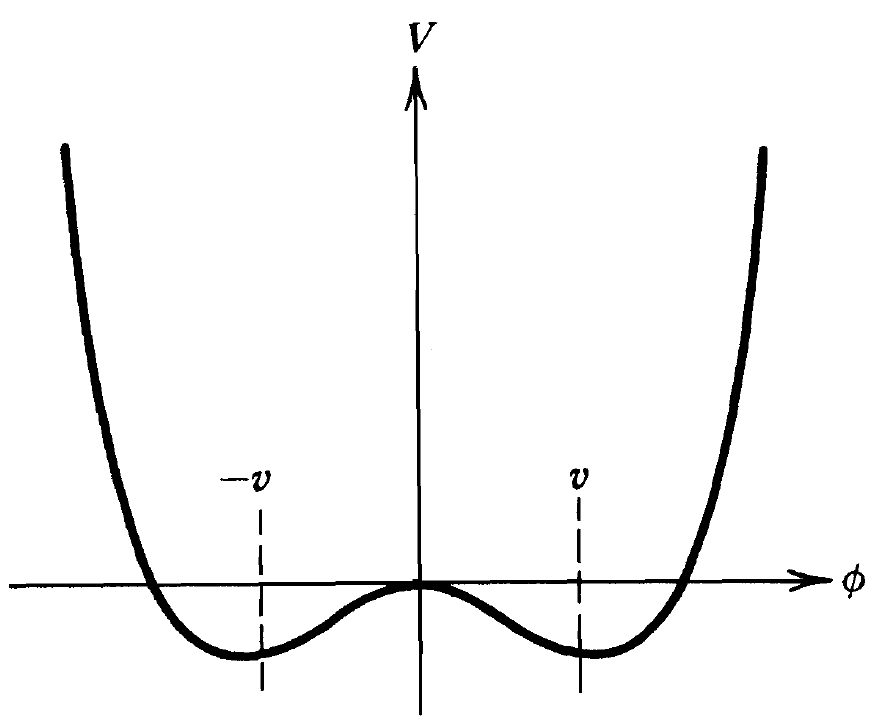
\includegraphics[width=0.5\textwidth]{figures/theory/Higgs_Field.png}
\caption{An example of one dimension ``Higgs'' potential \cite{Quark_Lepton}.}
  \label{fig:Higgs_Potential}
 \end{center}
\end{figure} 

In perturbative calculation we should involve expansions around the minimum energy and this can be done by expanding the $\phi$ around the $v$
$$\phi(t,\mathbf{x})=v+h(t,\mathbf{x}).$$
It means $\phi$ can be expressed by $h$, while potential $V$ will not be symmetry under the change of $h$ to $-h$. This makes the ``spontaneous symmetry breaking'' of $\phi$. After expanding the $\phi$ around the VEV, in new Lagrangian we have a term related to the mass of $h$ (actually is the mass of ``Higgs'' boson) and a term related to the masses of gauge bosons which means the gauge bosons obtained the masses. By the way, the masses of fermions in SM are also ``generated'' by Higgs mechanism.

Last but not least, the only $SU(2)_L$ local symmetry does not create the physical $\mathrm{Z}$ boson. It is created together with $\mathrm{W^{\pm}}$ and photon in $SU(2)_L \times U(1)_Y$ (``Y'' means hypercharge, $Y=2Q-T^{3}$ with $Q$ is the charge of particle, $T^3$ is third component of weak-isospin) symmetry which is proposed by Weinberg, Salam, and Glashow \cite{PhysRevLett.19.1264,Salam1959,GLASHOW1959107}. This $SU(2)_L \times U(1)_Y$ gauge invariance theory unifies electromagnetic and weak interactions and is called electroweak theory. Finally, the complete SM theory is based on $SU(3)_c \times SU(2)_L \times U(1)_Y$ gauge symmetry.



  

